\begin{framed}

Objetivos:
\begin{itemize}
    \item Encontrar expresiones para la velocidad, espesor de capa límite y coeficiente de fricción cuando el flujo en la capa límite es turbulento. 
\end{itemize}

Contenidos:
\begin{itemize}
    \item Expresiones de capa límite turbulenta para perfil supuesto.
    \item La ley de pared. 
\end{itemize}

Bibliografía:
\begin{itemize}
    \item Fox, R. W., Pritchard, P. J. y McDonald, A. T. (2009) Introduction to Fluid Mechanics. John Wiley \& Sons. Sección 9.5.
    \item White, F. M. (2006) Viscous Fluid Flow. McGraw-Hill. Tercera edición. Sección 6.4.
\end{itemize}
\end{framed}

\section*{Capa límite turbulenta}

En clases anteriores hemos estado analizando la capa límite de diferentes maneras usando von Kármán, Blasius, Flakner-Skan, y considerando succión y soplido.
Todos estos análisis tienen una cosa en común: la capa límite es considerada laminar.
Ya vimos también que el número de Reynolds en el caso de placa plana es variable en el espacio, y va subiendo a medida que nos movemos por la placa ($Re_x=U_\infty x/\nu$).
Ya sabemos que a medida que crece el número de Reynolds, el flujo se torna inestable, y ante cualquier perturbación se desencadena la transición a turbulencia.
Debido a esto, en la capa límite sobre una placa plana tendremos coexistirá flujo laminar (al incio de la placa) y flujo turbulento (aguas abajo), y en general se considera el Reynolds crítico como $Re_{cr} = 5\cdot10^{5}$.
Un ejemplo de esto se ve en la Figura \ref{fig:capa_limite_Re}, donde la capa límite se pega un salto cuando pasa de laminar a turbulenta, y en la parte turbulenta aparece una región denominada subcapa viscosa o laminar.
%
\begin{figure}
\centering
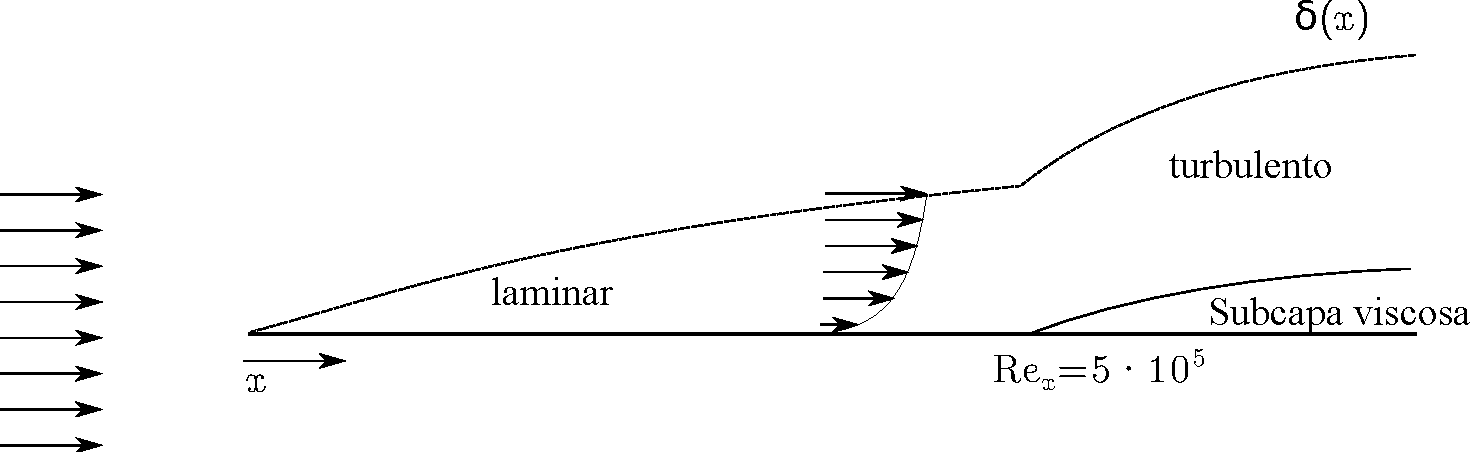
\includegraphics[width=0.9\textwidth]{clase09/capa_limite_Re.pdf}
\caption{Representación gráfica de la capa límite y su transición a turbulencia.}
\label{fig:capa_limite_Re}
\end{figure}

En esta clase vamos a analizar la capa límite turbulenta más en detalle.

\subsection*{Perfil de velocidad dado}

Así como vimos hace algunas clases cuando estudiamos turbulencia, sabemos que el perfil de velocidades va a ser bastante más desordenado en el caso laminar.
Es más, la velocidad va a ir variando con respecto a un promedio $\overline{u}$ debido a fluctuaciones turbulentas $u'$\footnote{Vean el siguiente video desde el minuto 18:40: \url{https://www.youtube.com/watch?v=wMxK2GtFFq0}}, lo que hace muy difícil su análisis.

Experimentalmente, se ha visto que la velocidad promedio de la capa límite turbulenta se acerca mucho a un perfil $y^{1/7}$, más específicamente:
%
\begin{equation}\label{eq:perfil_turbulento}
\frac{u}{U_\infty} = \left(\frac{y}{\delta}\right)^{1/7}.
\end{equation}
%
La Figura \ref{fig:capa_limite_turbulenta} compara la capa límite de Blasius, von Kármán ($\sim y^2$) y turbulenta ($\sim y^{1/7}$), donde el punto negro denota donde está el fin de la capa límite. Como pueden ver, el perfil turbulento tiene una gradiente mucho mayor al perfil laminar cerca de la pared, por lo tanto, el esfuerzo de pared ($\tau_w$) será mayor.
Cabe destacar que este no es un gran modelo cerca del fin de la capa límite, donde la gradiente no permite una transición suave al flujo uniforme al infinito.
%
\begin{figure}
\centering
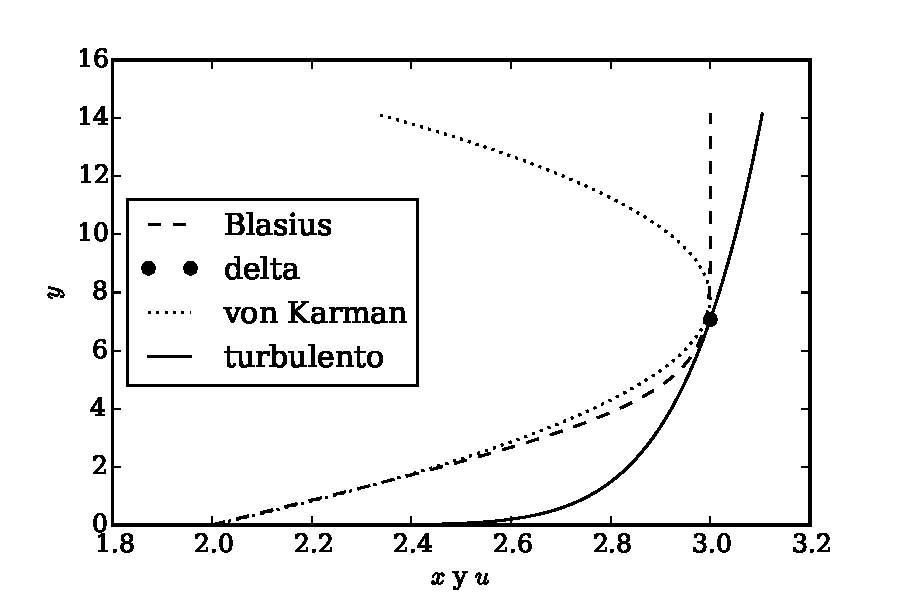
\includegraphics[width=0.6\textwidth]{clase11/capa_limite_turbulenta.pdf}
\caption{Perfil de capa límite laminar (Blasius y von Kármán) y turbulenta.}
\label{fig:capa_limite_turbulenta}
\end{figure}

Durante las últimas clases, hemos estado buscando expresiones para $\delta$, $\delta^*$, $\theta$ y $C_f$ para cada forma de modelar la capa límite. 
Esta no es la excepción, e intentaremos encontrar estas expresiones para el caso turbulento.
Debido a que estamos asumiendo un perfil de velocidades, este análisis debiese ser equivalente al de von Kármán cuando asumimos el perfil parabólico.
En ese caso, igualamos los esfuerzos de pared calculados con la relación integral de von Kármán:
%
\begin{equation}\label{eq:integral_vK}
\tau_w = \rho U_\infty^2 \frac{d\theta}{dx}
\end{equation}
%
donde $\theta$ es el espesor de momentum, a la ecuación de Newton $\tau_w = \left.\mu\frac{du}{dy}\right|_0$, sin embargo, al sacar la derivada de la Ec. \eqref{eq:perfil_turbulento} obtenemos
%
\begin{equation}
\tau_w = \left.\mu \frac{d}{dy}\left(U_\infty\frac{u}{\delta}\right)^{1/7}\right|_0 = \left.\frac{U_\infty\mu}{\delta^{1/7}}y^{-6/7}\right|_0 = \infty.
\end{equation}
%
Claramente, tenemos un problema con el perfil escogido, y vamos a tener que sacar $\tau_w$ de otra manera.
La forma más fácil es hacer un símil con flujo en tuberías, y usar el resultado de $\tau_w$ de ahí para igualarlo a la ecuación integral de momentum de von Kármán.
En este símil, la velocidad al infinito ($U_\infty$) será la velocidad al centro de la tubería, por lo tanto, $\delta=R$.
Partamos analizando el volumen de control de la Figura \ref{fig:volumen_control}, de ancho $dx$ que ocupa toda la sección transversal de la tubería.
Aplicando el principio de conservación de la cantidad de movimiento, los flujos se cancelan por continuidad, las únicas fuerzas son por la presión y el esfuerzo de pared y quedamos con
%
\begin{align}\label{eq:deltap_tuberia}
\Delta p\pi R^2 &= \tau_w2\pi Rdx\nonumber\\
\Delta p &= \frac{2\tau_w dx}{R}.
\end{align}
%
\begin{figure}
\centering
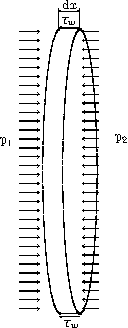
\includegraphics[width=0.2\textwidth]{clase11/volumen_control.pdf}
\caption{Volumen de control en una tubería.}
\label{fig:volumen_control}
\end{figure}

Por otra parte, del estudio de flujo en tuberías sabemos que un Bernoulli modificado entre $1$ y $2$ da que la caída de presión es solamente debido a la altura de pérdidas:
%
\begin{equation}\label{eq:perdida_altura}
\frac{\Delta p}{\rho} = h_L g = f \frac{dx}{D}\frac{\overline{V}^2}{2}.
\end{equation}
%
Reemplazando la Ec. \eqref{eq:deltap_tuberia} en la Ec. \eqref{eq:perdida_altura}, nos deja
%
\begin{equation}
\tau_w = \frac{f}{8}\rho\overline{V}^2
\end{equation}

El factor $f$ es el factor de fricción.
En Mecánica de Fluidos General aprendimos que hay muchas formas de calcular $f$: a través del diagrama de Moody, o con las ecuaciones de Haaland, Colebrook, Blasius, etc.
Usemos la ecuación de Blasius, que tiene la ventaja de ser explícita, y válida hasta $Re=10^5$ (ojo: $Re$, no $Re_x$):
%
\begin{equation}
f = \frac{0.316}{Re^{1/4}}
\end{equation}
%
y reemplazando quedamos con 
%
\begin{equation}\label{eq:tau_tuberia}
\tau_w = \frac{0.0395\rho\overline{V}^2}{Re^{1/4}} = \frac{0.0332\rho\overline{V}^2}{\left(\frac{R\overline{V}}{\nu}\right)^{1/4}}
\end{equation}

Acordémonos que estamos haciendo el simil de flujo sobre una placa con flujo en tubería, y sobre la placa, la velocidad que nos interesa es $U_\infty$, correspondiente a la velocidad en el centro de la tubería $U_c$.
Para parar los valores de $\overline{V}$ a $U_c=U_\infty$ en la Ec. \eqref{eq:tau_tuberia} podemos usar el caudal:
%
\begin{equation}
Q = \overline{V}A = \int_0^Ru2\pi r dr.
\end{equation}
%
Si reemplazamos en esta ecuación que $u=U\infty(y/\delta)^{1/7}$, y que $y=R-r$ llegamos a
%
\begin{align}
\overline{V}A=2\pi U_\infty\int_0^R\left(1-\frac{r}{R}\right)^{1/7}rdr = \frac{49}{120}R^22\pi U_\infty\nonumber\\
\Rightarrow \overline{V} = U_\infty\frac{49\cdot2\pi R^2}{120\pi R^2} = 0.817 U_\infty.
\end{align}
%
Sabiendo que $R=\delta$, podemos reescribir la Ec. \eqref{eq:tau_tuberia} como
%
\begin{equation}\label{eq:tau_placa}
\tau_w = \frac{0.0332\rho(0.817 U_\infty)^2}{\left(\frac{\delta0.817 U_\infty}{\nu}\right)^{1/4}} = 0.0233\rho U_\infty^2\left(\frac{\nu}{\delta U_\infty}\right)^{1/4}
\end{equation}

La Ec. \eqref{eq:tau_placa} está mucho mejor, ya que $\tau_w$ no es infinito como cuando usamos la ley de viscosidad de Newton.
Igualemos la Ec. \eqref{eq:tau_placa} a la relación integral de von Kármán (Ec. \eqref{eq:integral_vK}):
%
\begin{align}\label{eq:delta_turb}
\tau_w = \rho U_\infty^2\frac{d\theta}{dx} &= \rho U_\infty^2 \frac{d}{dx}\left[\int_0^\delta \frac{u}{U_\infty}\left(1-\frac{u}{U_\infty}\right)dy\right]\nonumber\\
0.0233 \left(\frac{\nu}{\delta U_\infty}\right)^{1/4} &= \frac{d}{dx}\left[\int_0^\delta \frac{u}{U_\infty}\left(1-\frac{u}{U_\infty}\right)dy\right] = \frac{d}{dx}\left[\frac{7}{72}\delta\right]\nonumber\\
\Rightarrow 0.0233\cdot\frac{72}{7}\left(\frac{\nu}{U_\infty}\right)^{1/4} dx &= \delta^{1/4}d\delta\nonumber\\
\delta^{5/4} &= \frac{0.3}{\left(\frac{U_\infty x}{\nu}\right)^{1/4}}x^{5/4}\nonumber\\
\frac{\delta}{x} &= \frac{0.382}{Re_x^{1/5}}
\end{align}

Por otra parte, de la Ec. \eqref{eq:tau_placa} tenemos el esfuerzo sobre la placa plana y el valor de $\delta$ con la Ec. \eqref{eq:delta_turb}, y el coeficiente de fricción es
%
\begin{align}
c_f &= \frac{\tau_w}{\frac{1}{2}\rho U_\infty^2} = \frac{0.0233\rho U_\infty^2\left(\frac{\nu}{\delta U_\infty}\right)^{1/4}}{\frac{1}{2}\rho U_\infty^2 }\nonumber\\
    &= 0.0466\left(\frac{\nu}{\delta U_\infty}\right)^{1/4} = 0.0466\left(\frac{\nu}{\frac{0.382x}{Re_x^{1/5} U_\infty}}\right)^{1/4} \nonumber\\
    &= \frac{0.0594}{Re_x^{1/5}}
\end{align}

Además, podemos integrar la ecuación para espesor de desplazamiento usando el perfil de velocidad $\sim y^{1/7}$ para obtener
%
\begin{equation}
\frac{\delta^*}{x}=\frac{0.0463}{Re^{1/5}} 
\end{equation}

\subsection*{Ley de pared}

Así como en el análisis de von Kármán para el caso laminar, uno podría alegar que el asumir un perfil de velocidad es poco riguroso (sobre todo en el caso turbulento), pero funciona bastante bien.
En todo caso, podemos hacer un análisis más detallado, y con mayor trasfondo físico, para obtener u perfil de velocidades.
Ocurre que el comportamiento de la capa límite en la zona cercana a la pared (el primer $\sim20\%$ de $\delta$), tiene un comportamiento muy universal, que es independiente de si estamos frente a una placa plana, curva, una tubería, etc.

Para llegar a este comportamiento universal, primero debemos adimensionalizar las variables; usemos análisis dimensional para esto.
La primera pregunta es \mbox{?`}cuáles son las variables importantes? Las más fáciles son: $\mu$, $\rho$, $y$ y $u$.
En la zona cercana a la pared, el flujo externo está muy lejos, y consideraremos que $U_\infty$ no es una variable importante en el problema, eso si, al estar la placa cerca, $\tau_w$ es importante.
Quedamos entonces con $5$ parámetros importantes, que se describen por $3$ unidades dimensionales básicas (T,L,M), y el problema se describe usando solamente dos variables adimensionales.
Usando el teorema de Buckingham, llegamos a los siguientes parámetros adimensionales:
%
\begin{align}
u^+ = u\sqrt{\frac{\rho}{\tau_w}}\nonumber\\
y^+ = \frac{y}{\nu}\sqrt{\frac{\tau_w}{\rho}}
\end{align}
%
y si definimos $u_\tau=\sqrt{\tau_w/\rho}$ podemos reescribir los parámetros adimenisonales como
%
\begin{align}\label{eq:unidades_pared}
u^+=\frac{u}{u_\tau}\nonumber\\
y^+=\frac{yu_\tau}{\nu}.
\end{align}
%
Las variables $u^+$ y $y^+$ son la velocidad y distancia en \emph{unidades de pared}.

Recordemos un poco de lo que aprendimos estudiando turbulencia.
Cuando el flujo es turbulento, conviene usar la ecuación de Navier-Stokes promediada, que conocemos como ecuación RANS (Reynolds Averaged Navier-Stokes):
%
\begin{equation}\label{eq:RANS}
\frac{\partial \overline{u}_i}{\partial t} + \overline{u}_j\frac{\partial \overline{u}_i}{\partial x_j}  = -\frac{1}{\rho}\frac{\partial \overline{p}}{\partial x_i} + \frac{\partial}{\partial x_j}\left(\nu \frac{\partial \overline{u}_i}{\partial x_j} - \overline{u'_iu'_j}\right).
\end{equation}
%
Hagamos las siguientes aproximaciones y consideraciones:
%
\begin{itemize}
\item $\overline{u} >> \overline{v}$, $\overline{w}$
\item $\frac{\partial}{\partial y} >> \frac{\partial}{\partial x}$, $\frac{\partial}{\partial z}$
\item Flujo estacionario
\item Presión constante
\end{itemize}
%
Las primera aproximación de la lista viene simplemente de decir que, en promedio, el flujo tiene una dirección claramente preferente: la dirección $x$.
Por otra parte, la segunda es que la variación de velocidad en la dirección $y$ (alejándose de la placa) es muchísimo más rápida que en la dirección del flujo y en la dirección perpendicular.
Aplicando esas consideraciones, y la ecuación de continuidad, la Ec. \eqref{eq:RANS} en la dirección $x$ se simplifica a 
%
\begin{equation}
\nu\frac{\partial^2 \overline{u}}{\partial y^2} - \frac{\partial \overline{u'v'}}{\partial v} = 0.
\end{equation}
%
Adimensionalizando con $u_\tau$, llegamos a
%
\begin{align}
\nu\frac{\partial^2\overline{u^+}u_\tau}{\partial y^{+2}\left(\frac{u_tau}{\nu}\right)^2} - \frac{\partial \overline{u^{+\prime}v^{+\prime}}}{\partial y^+\frac{u_\tau}{\nu}}u_\tau^2 = 0\nonumber\\
\frac{\partial^2\overline{u^+}}{\partial y^{+2}}-\frac{\partial \overline{u^{+\prime}v^{+\prime}}}{\partial y^+} = 0\nonumber\\
\frac{\partial}{\partial y^+}\left(\frac{\partial\overline{u^+}}{\partial y^+}-\overline{u^{+\prime}v^{+\prime}}\right) = 0
\end{align}
%
e integrando queda
%
\begin{equation}\label{eq:uplus_aux}
\frac{\partial\overline{u^+}}{\partial y^+}-\overline{u^{+\prime}v^{+\prime}}= C_0
\end{equation}

El valor de $C_0$ no es importante, y podemos elegit $C_0=1$.
La Ec. \eqref{eq:uplus_aux} muestra que la fuerza en un elemento de fluido el equilibrio entre las fuerzas viscosas ($\partial \overline{u^+}/\partial y^+$ esta relacionada con el esfuerzo de un fluido Newtoniano), y el esfuerzo de Reynolds (acuérdense de la interpretación de $\overline{u'_iu'_j}$ como un esfuerzo).
Veamos dos casos extremos:

\paragraph*{Flujo cerca de la pared.} En este caso, los esfuerzos viscosos debido a la presencia de la pared van a dominar sobre los esfuerzos turbulentos:
%
\begin{align}
&\frac{\partial\overline{u^+}}{\partial y^+} >> \overline{u^{+\prime}v^{+\prime}}\nonumber\\
&\Rightarrow \frac{\partial\overline{u^+}}{\partial y^+} = 1.
\end{align}
%
Integrando, llegamos a
%
\begin{equation}\label{eq:subcapa_viscosa}
\overline{u^+} = y^+.
\end{equation}
%
La zona de la capa límite que se comporta de esta manera lineal es la subcapa viscosa (vean la Figura \ref{fig:capa_limite_Re}).

\paragraph*{Flujo alejado de la pared.} En este caso, la pared está suficientemente lejos que el esfuerzo viscoso no es importante:
%
\begin{align}
&\frac{\partial\overline{u^+}}{\partial y^+} << \overline{u^{+\prime}v^{+\prime}}\nonumber\\
&\Rightarrow \overline{u^{+\prime}v^{+\prime}} = 1.
\end{align}
%
Hay que tener en consideración que, a pesar que llamamos a esta zona ``lejos'', sigue estando dentro de la zona \emph{interna} de la capa límite (bajo el primer 20\%).
Este caso es un poco más complicado, ya que no sabemos como se comportan las fluctuaciones.
La forma de enfrentar esto es usando modelos que representen el efecto de las fluctuaciones.
El modelo más simple es representar el esfuerzo de Reynolds usando el concepto de viscosidad turbulenta (acuérdense de las clases de turbulencia!):
%
\begin{equation}\label{eq:visc_turb}
\overline{u'v'} = \nu_t \frac{\partial\overline{u}}{\partial v}.
\end{equation}
%
Adimensionalicemos esta ecuación:
%
\begin{align}
\overline{u^{+\prime}v^{+\prime}} = \nu_t \frac{\partial\overline{u}}{\partial v}\frac{1}{u_\tau^2} = 1\nonumber\\
\Rightarrow u_\tau^2 = \nu_t \frac{\partial \overline{u}}{\partial y}
\end{align}
%
Ahora necesitamos un modelo para representar $\nu_t$.
El más básico que estudiamos era el modelo de longitud de mezcla de Prandtl:
%
\begin{equation}\label{eq:long_mezcla}
\nu_t = l_m^2\left|\frac{\partial\overline{u}}{\partial y}\right|,
\end{equation}
%
y reemplazando en la Ec. \eqref{eq:visc_turb} llegamos a
%
\begin{align}
u_\tau^2 &= l_m^2\left|\frac{\partial\overline{u}}{\partial y}\right|\frac{\partial\overline{u}}{\partial y} \nonumber\\
\Rightarrow u_\tau &= l_m\frac{\partial\overline{u}}{\partial y}.
\end{align}
%
Esto parece un argumento circular, ya que, a pesar que tenemos una expresión para $\nu_t$, necesitamos un modelo para determinar $l_m$. 
En flujo sobre una placa plana, es sabido que $l_m=\kappa y$ funciona bien, lo que nos deja con
%
\begin{equation}
u_\tau = \kappa y \frac{\partial\overline{u}}{\partial y}
\end{equation}
%
y si adimensionalizamos esta ecuación, quedamos con:
%
\begin{align}
u_\tau &= \kappa y^+\frac{\nu}{u_\tau} \frac{\partial\overline{u^+}u_\tau}{\partial y^+ \frac{\nu}{u_\tau}}\nonumber\\
\Rightarrow 1&= \kappa y^+ \frac{\partial\overline{u^+}}{\partial y^+}\nonumber\\
\frac{1}{\kappa}\frac{\partial y^+}{y^+} &= \partial u^+.
\end{align}
%
Integrando, quedamos con
%
\begin{equation}\label{eq:ley_pared}
u^+ = \frac{1}{\kappa}\ln(y^+) + B,
\end{equation}
%
que se conoce como la ley de pared.
En general, $\kappa=0.41$ y $B=5$ son los valores más aceptados para las constantes en la Ec. \eqref{eq:ley_pared}.
La ley de pared tiene un carácter universal, ya que se cumple tanto en flujo cobre una placa plana, como dentro de una tubería o en placas curvas.

La gráfica en la Figura \ref{fig:ley_pared} demuestra lo cercana que está la ley de pared de experimentos, y nos confirma que el modelo $l_m = \kappa y$ funciona muy bien.
%
\begin{figure}
\centering
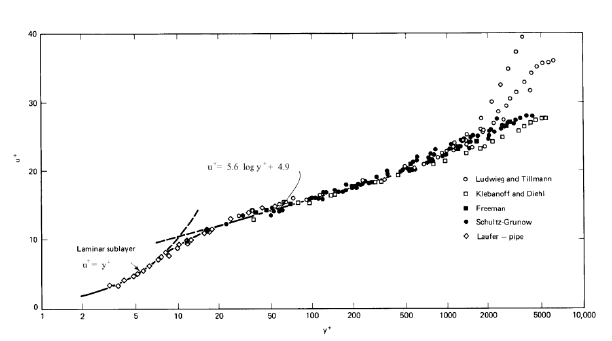
\includegraphics[width=0.7\textwidth]{clase11/ley_pared.png}
\caption{Comparación de la ley de pared con experimentos. Gráfica obtenida de Clauser, Francis H. ``The turbulent boundary layer.'' Advances in applied mechanics 4 (1956): 1-51.}
\label{fig:ley_pared}
\end{figure}
